\section{Background}
This chapter explains the necessary background to understand Scala and code formatting.
More specifically, we motivate why Scala presents an interesting challenge for code formatters.
We go into details on Scala's rich syntax and popular idioms that introduced unique challenges to the design of scalafmt.
We follow up with a brief history on code formatters for both Scala as well as other programming languages.
We will see that although code formatters have a long history, the last 5 years have brought a lot of research in optimization based formatters, which scalafmt's design takes inspiration from.

\subsection{Scala the programming language}
Scala\autocite{odersky_scala_2004} is a general purpose programming language that was first released in 2004.
Scala combines features from object-oriented and functional programming paradigms, allowing maximum code reuse and extensibility.

Scala can run on multiple platforms.
Most commonly, Scala programs compile to bytecode and run on the JVM.
With the releases of Scala.js\autocite{doeraene_scala.js_2015}, JavaScript has recently become a popular target platform for Scala developers.
Even more recently, the announcement of Scala Native\autocite{_scala-native/scala-native_????} shows that LLVM and may become yet another viable platform for Scala developers.

Scala is a popular programming language.
The Scala Center estimates that more than half a million developers are using Scala\autocite{odersky_scala_2016}.
Large organizations such as Goldman Sachs, Twitter, IBM and Verizon run Scala code in production systems.
The 2015 Stack Overflow Developer Survey shows that Scala is the 6th most loved technology and 4th best paying technology to work with\autocite{_stack_????}.
The popularity of Apache Spark\autocite{_apache_????-1}, a cluster computing framework for large-scala data processing, has made Scala a language of choice for many developers and scientists working in big data and machine learning.

Scala is a programming language with rich syntax and many idioms.
The following chapters discuss in detail several prominent syntactic features and idioms of Scala.
Most importantly, we highlight coding patterns that encourage developers to write larger statements instead of many small statements.
In section~\ref{sec:algorithms}, we explain why large statements introduce a challenge to code formatting.

\subsubsection{Higher order functions}
Higher order functions (HOFs) are a common concept in functional programming languages and mathematics.
HOFs are functions that can take other functions as arguments and can return functions as return values.
Languages that provide a convenient syntax to manipulate HOFs are said to make functions first-class citizens.

Functions are first-class citizens in Scala.
Consider listing~\ref{lst:hof}.
\lstinputlisting[label={lst:hof}, float, caption=Higher order functions]{code/hof.scala}
The method \texttt{twice} takes an argument \texttt{f}, which is a function from an integer to an integer.
The method returns a new function that will apply \texttt{f} twice to an integer argument.
This small example takes advantage of several syntactic conveniences provided by Scala.
For example, in line 2 the argument \texttt{\_ + 3} creates a new \texttt{Function[Int, Int]} object.
The function call \texttt{f(x)} is in fact sugar for the method call \texttt{f.apply(x)} on a \texttt{Function[Int, Int]} instance.
Listing~\ref{lst:hof_nosugar} shows an equivalent program to listing~\ref{lst:hof} without syntactic sugar.
\lstinputlisting[label={lst:hof_nosugar}, float, caption=Higher order functions without syntactic sugar]{code/hof-nosugar.scala}
Observe that what was expressed as a single statement in line 1 of listing~\ref{lst:hof} is expressed with multiple statements in lines 1 and 2 of listing~\ref{lst:hof_nosugar}.

\subsubsection{Immutability}
Functional programming encourages stateless functions which operate on immutable data structures and objects.
An immutable object is an object that once initialized, cannot be modified.
Immutability offers several benefits to software development in areas including concurrency and testing.
Listing~\ref{lst:immutable} shows an example of manipulating an immutable list.
\lstinputlisting[label={lst:immutable}, float, caption=Manipulating immutable list]{code/immutable.scala}
Note that each \texttt{map} and \texttt{filter} operation creates a new copy of the list with the modified contents.
The original list remains unchanged.
Listing~\ref{lst:mutable} show the equivalent operation using a mutable list.
\lstinputlisting[label={lst:mutable}, float, caption=Manipulating mutable list]{code/mutable.scala}
Observe that what was listing~\ref{lst:immutable} is a single statement while listing~\ref{lst:mutable} is multiple statements.

\subsubsection{SBT build configuration}
SBT\autocite{_sbt_????} is an interactive build tool used by many Scala projects.
SBT configuration files are written in \texttt{*.sbt} or \texttt{*.scala} files using Scala syntax and semantics.
Although SBT configuration files use plain Scala, they typically use coding patterns which are different from traditional Scala programs.
Listing~\ref{lst:sbt} is an example project definition in SBT.
\lstinputlisting[label={lst:sbt}, float, caption=SBT project definition]{code/sbt.scala}
Observe that the project is defined as a single statement and makes extensive use of symbolic infix operators.
Due to the nature of build configurations, argument lists to can becomes unwieldy long and a single project statement can span up to dozens or even hundreds of lines of code.

% \subsection{Metaprogramming with scala.meta}
% Scala.meta\autocite{_scala.meta_????} is a robust and portable metaprogramming toolkit for Scala.
% Scala 2.10 compiler introduced the first metaprogramming API for Scala via compile-time macros and runtime reflection.
% Library authors could take advantage of this new functionality to implement more advanced features in their libraries.
% However, the Scala compiler metaprogramming facilities exposed compiler internals to its users.

\subsection{Code formatters}
%
% In the literature, the term \emph{pretty-printer} is more commonly used than code formatter.
% This thesis uses code formatter the terms are used interchangeably and the author does not distinguish between the two.} 
% We emphasize formatters that support line length length limits.
% As future sections discuss, line length limits turn out to be a big challenge to implement.

In this chapter, we look at a variety of code formatters that have been developed.

\subsubsection{Natural language}
The science of displaying aesthetically pleasing text predates as early as 1956\autocite{harris_keyboard_1956}.
The first efforts involved printing natural language text and finding the right places to insert carriage returns to break long lines.
As soon as programming languages evolved, software developers began to apply the similar ideas to source code.

LaTeX


\subsubsection{ALGOL 60}
Scowen\autocite{scowen_soapprogram_1971} developed SOAP in 1971, a code formatter for ALGOL 60.
The main motivation for SOAP was to make it ``easier for a programmer to examine and follow a program'' as well as to maintain a consistent coding style.
This motivation is still relevant in modern software development.
SOAP did provide a line length limit.
However, SOAP would fail execution if the provided line length turned out to be too small.
With hardware from 1971, SOAP could format 600 lines of code per minute.

\subsubsection{LISP}
In 1973, Goldstein\autocite{goldstein_pretty-printing_1973} explored code formatting algorithms for LISP\autocite{mccarthy_recursive_1960} programs.
LISP is a family of programming languages and is famous for it's parenthesized prefix notation.
Listing~\ref{lst:lisp} shows a program in LISP to calculate factorial numbers.
\lstinputlisting[label={lst:lisp}, float, caption=A LISP program]{code/lisp.lisp}
The simple syntax, extensive use of parentheses and nested nature of LISP programs makes them an excellent ground to study code formatters.

Goldstein presented a \emph{recursive re-predictor} algorithm in his paper.
The recursive re-predictor algorithm runs a top-down traversal on the abstract syntax tree of a LISP program.
While visiting each node, the algorithms tries to first obtain a \emph{linear-format}, i.e. fit remaining body on a single line.
If there isn't enough space on the line to fit a linear format, the algorithm falls back to \emph{standard-format} where each argument is put on a separate line aligned by the first argument.
Goldstein observes that this algorithm is practical despite the fact that its running time is exponential in the worst cases.
Bill Gosper used the re-predictor algorithm to implement GRINDEF\autocite{_bill_????}, one of the first code formatters for LISP.
Goldstein's contributions extend beyond formatting algorithms.
Firstly, in his paper he studies how to format comments.
Secondly, he presents several different formatting layouts which can be configured by the users.
Both of those concerns are relevant for modern code formatters.

\subsubsection{Language agnostic}\label{sec:agnostic}
Derek C. Oppen pioneered the work on language agnostic code formatting in 1980\autocite{oppen_prettyprinting_1980}.
Oppen presented an algorithm is not tied to particular programming language.
The algorithms runs in linear time to the size of the input program and is incredibly memory efficient.
Users provide a preprocessor to integrate the algorithm with a particular programming language.
Besides impressive performance results, Oppen claims that a key feature of the algorithms is its streaming nature.
The algorithm prints formatted lines as soon as they are input instead of waiting until the entire input stream has been read.
However, Oppen's algorithm shares a worrying limitation with SOAP: it cannot handle the case when the line length is insufficiently large.

Mark van der Brand presented a library could generate a formatter given a context-free grammar\autocite{van_den_brand_generation_1996}.
Brand correctly identifies that the development of code formatters requires a lot of effort and a generic solution may be possible.
Beyond the usual motivations for developing code formatters, Brand mentions that formatters ``relieve documentation writers from typesetting programs by hand''.
The focus on documentation is reflected by the fact that generated formatter could produce both ASCII formatted code as well at \LaTeX{} formatted code.
Since comments are typically not included a syntax tree, the presented algorithm has an elaborate scheme to infer the location of comments in the produced output.
Like Oppen's algorithm, this library requires the user to translate code from a particular programming language into the library's constructs.
Unlike Oppen's algorithm, Brand does not consider line length limits in his algorithm.

John Hughes extended on Oppen's work on language agnostic formatting in term of programming techniques\autocite{hughes_design_1995}.
Hughes presented a design of a \emph{pretty-printing} library that leverages the functional programming paradigm.
Hughes says his library is a pretty-printer and not code formatters since the library does not consider how to format existing source code.
Instead, the library prints data structures directly from their values.
Wadler\autocite{wadler_prettier_2003} and Chitil\autocite{swierstra_linear_2009} extend on Hughes's and Oppen's work.
However, only in term of functional programming techniques instead of formatting or layout algorithms.

% More recently, Bagge and Hasu extend on Wadlers work in a language agnostic \emph{pipeline} for formatters\autocite{bagge_pretty_2013}.
% The main motivation for this work was to increase modularity and composability of format

\subsubsection{clang-format}
Daniel Jasper triggered a new trend in optimization based coded formatters with the release of \emph{ClangFormat}\autocite{jasper_clang-format_2014} in 2013.
ClangFormat is a code formatter for C, C++, Java, JavaScript, Objective-C and Protobuf code.
Figure~\ref{fig:clang_format} shows the architecture of ClangFormat.
\begin{figure}
  \centering
  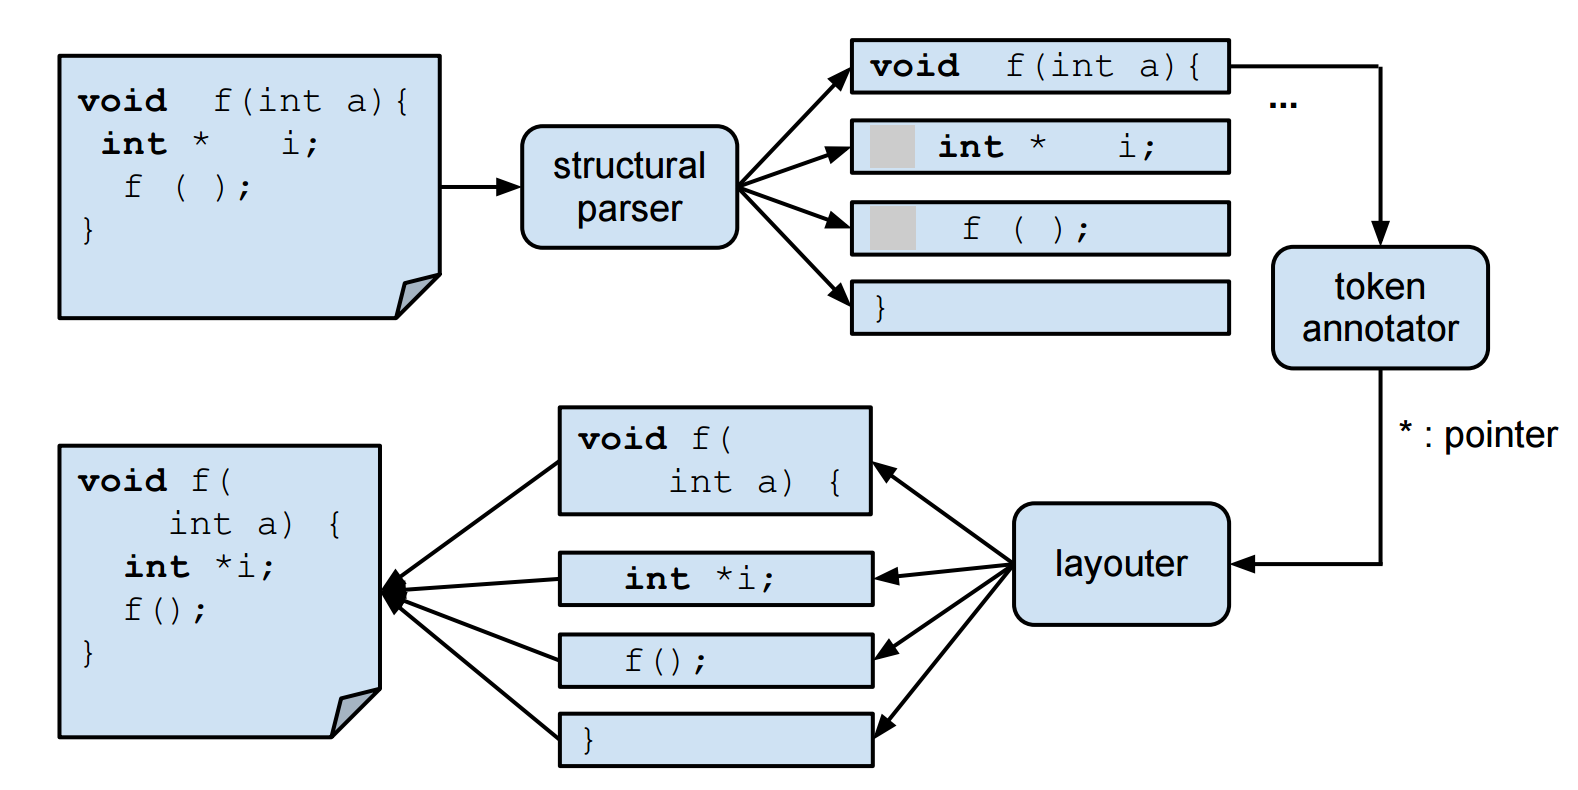
\includegraphics[width=0.9\textwidth]{img/clang-format.png}
  \caption{ClangFormat architecture}
  \label{fig:clang_format}
\end{figure}
The main components are the \emph{structural parser} and the \emph{layouter}.

ClangFormat employs a structural parser to split source code into a sequence of \emph{unwrapped-lines}.
An unwrapped line is a statement that should fit on a single line if given sufficient line length.
A key feature of unwrapped lines is that they should not influence other unwrapped lines.
The parser is lenient and parses even syntactically invalid code.
The parsed unwrapped lines are passed onto the layouter.

The ClangFormat layouter uses a novel approach to implement line wrapping.
Each line break is assigned a penalty according to several rules such as nesting and token type.
At each token, the layouter can choose to continue on the same line or break.
This forms an acyclic weighted directed graph with the first token of an unwrapped line being the root and all paths ending at the last token of the unwrapped line.
The layouter employs Dijkstra's\autocite{dijkstra_note_1959} shortest path algorithm to find the layout that has the lowest penalty.
To guarantee good performance, the layouter uses several domain specific optimizations to cut the search space.

Despite being seemingly language independent, ClangFormat does leverage the language agnostic formatting techniques described section~\ref{sec:agnostic}.
Support for each language has been added as ad-hoc extensions to the ClangFormat parser and layouter.
ClangFormat supports a variety of configuration options, include 6 configurations based on published style guides from Google, LLVM and several other large organizations.

A notable feature of ClangFormat is that it's opinionated.
ClangFormat makes a best effort to format even the most egregiously formatted input.
Listing~\ref{lst:clang_opinion} shows an offensively formatted C++ code snippet.
\lstinputlisting[label={lst:clang_opinion}, float, caption=Unformatted C++ code]{code/terrible.cpp}
Listing~\ref{lst:clang_opinion2} shows the same snippet after being formatted with ClangFormat.
\lstinputlisting[label={lst:clang_opinion2}, float, caption=ClangFormat formatted C++ code]{code/target/unterrible.cpp}
ClangFormat is opinionated in the sense that it does not respect the user's line breaking decisions.
This feature makes it possible to ensure that all code follows the same style guide, regardless of author.

\subsubsection{dartfmt}
Dartfmt\autocite{nystrom_dart_style_2014} is an opinionated code formatter for the Dart programming language, developed at Google.
Like ClangFormat, dartfmt has a line length setting and is opinionated.
Bob Nystrom, the author of dartfmt, discusses the design of dartfmt in an excellent post\autocite{nystrom_hardest_2015} on his blog.
In his post, Nystrom cites Knuth's work on \LaTeX{} to argue that the design of a code formatters is significantly complicated by a column limit setting.
The line wrapping algorithm employs a \emph{best-first search}\autocite{pearl_heuristics:_1984},
a minor variant of the shortest path search in ClangFormat.
As with ClangFormat, a range of domain-specific optimizations were required to make the search scale for real-world code.
For example, listing~\ref{lst:dead_end} show a motivating case for the \emph{avoid dead ends} optimization.
\lstinputlisting[label={lst:dead_end}, float, caption=Avoid dead ends]{code/dead-end.dart}
Since the call to \texttt{firstCall} already fits on a line, there is no need to explore line breaks inside its argument list.
A textbook best-first search would explore a space of line breaks inside the \texttt{firstCall} argument list while the dartfmt optimized search is able to quickly eliminate such dead ends and break before the \texttt{"long argument string"} literal.


\subsubsection{gofmt}
Gofmt\autocite{gofmt94:online} is a code formatter for the Go programming language, developed at Google.
Gofmt is noteworthy for its heavy adoption by the Go programming community.
Moreover, gofmt has successfully been used to automatically migrate Go codebases from legacy versions to new source-incompatible releases.
However, gofmt does support neither a column limit nor an opinionated setting.
These limitations makes gofmt less interesting for the work presented in this thesis.

\subsubsection{rustfmt}
\subsubsection{scalariform}
Scalariform\autocite{russell_scalariform_2010} is a widely used code formatter for Scala.
Scalariform does an excellent job of tidying common formatting errors and it supports a variety of configuration options.
Scalariform is also impressively fast, it can format large files with over 4.000 lines of code in under 250 milliseconds on a modern laptop.

However, Scalariform lacks two key features: a line length and opinionated setting.
Firstly, the line length setting is necessary to implement many popular coding styles in the Scala community.
For example, the Spark\autocite{xin_spark_2015} and Scala.js\autocite{doeraene_scala.js_2015} coding styles have 100 character and 80 character column limits, respectively.
Second, the lack of an opinionated setting makes it impossible to enforce certain coding styles.
For example, the Scala.js coding style enforces \emph{bin-packing}, where arguments should be arranged compactly up to the column length limit.
Listings~\ref{lst:bin_pack} and~\ref{lst:non_bin_pack} shows an example of bin packing enabled and disabled, respectively.
\begin{minipage}{.45\textwidth}
  \lstinputlisting[label={lst:bin_pack}, caption=Bin-packing]{code/bin-pack.scala}
\end{minipage}
\hfil
\begin{minipage}{.45\textwidth}
  \lstinputlisting[label={lst:non_bin_pack}, caption=No bin-packing]{code/non-bin-pack.scala}
\end{minipage}
Scalariform has no setting to convert formatted code like in listing~\ref{lst:non_bin_pack} to the code in listing~\ref{lst:bin_pack}.
